\documentclass[11pt]{article}
\usepackage{graphicx, booktabs, amsmath, hyperref, geometry}
\usepackage[numbers]{natbib}
\geometry{margin=1in}

\title{\textbf{How Generative AI Shapes Student Academic Outcomes:\\
Study Displacement, Anxiety, Burnout, and Skill Retention}}

\author{Sanjiv Das\\
Santa Clara University\\
\texttt{srdas@scu.edu}}

\date{\today}

\begin{document}
\maketitle

%──────────────────────────────────────────────────────────────────
\begin{abstract}
Generative AI tools are rapidly entering higher education, yet their effects on
learning outcomes and student well-being remain contested. Using a large
cross-sectional dataset of 50{,}000 students spanning five major fields and four
academic years, this paper investigates three inter-related questions: (1)~Does
GenAI use displace traditional study time, and does that substitution affect
post-semester GPA? (2)~What factors best predict exam anxiety and burnout risk?
(3)~Does the \emph{quality} of AI use---measured by prompt engineering skill and
tool diversity---improve knowledge retention, and does institutional policy
moderate this effect? We find that GenAI usage exhibits a mild but significant
displacement of traditional study hours ($r = -0.16$) and that an inverted-U
relationship with GPA exists: moderate users (3--12~h/week) outperform both
abstainers and heavy users. Counterintuitively, institutions with strict AI bans
produce more anxious and burned-out students than those with permissive policies.
Finally, prompt engineering skill accounts for an 11-point gap in skill retention
scores (beginner: 71.1 vs.\ advanced: 82.1), while tool diversity provides an
additional monotonic benefit ($r = +0.20$). Together, these findings argue for
structured, permissive institutional policies paired with deliberate instruction
in AI-use skills.
\end{abstract}

%──────────────────────────────────────────────────────────────────
\section{Introduction}

The proliferation of large language model-based tools---ChatGPT, Claude, Gemini,
and their peers---has placed generative AI (GenAI) in the hands of millions of
students. Proponents argue that these tools democratize access to expert
knowledge, accelerate iteration on drafts, and free cognitive bandwidth for
higher-order reasoning. Critics worry that students who outsource effort to AI
will retain less knowledge, grow dependent, and face heightened anxiety when
forced to perform without assistance (e.g., on exams).

Empirical evidence at scale is still sparse. Most studies rely on self-reports
from small samples, focus on a single outcome, or conflate quantity of AI use
with quality of use. This paper addresses all three shortcomings using a
50{,}000-student dataset with rich behavioral, attitudinal, and performance
variables. We pursue three research questions (RQs):

\begin{description}
  \item[RQ1] Does weekly GenAI usage displace traditional study time, and does
    that substitution harm post-semester GPA?
  \item[RQ2] What factors---AI dependency, usage intensity, or institutional
    policy---best predict exam anxiety and burnout risk?
  \item[RQ3] Does ``smart'' AI use (high prompt engineering skill; broad tool
    diversity) improve skill retention, and does institutional policy moderate
    this effect?
\end{description}

The remainder of the paper is organised as follows. Section~\ref{sec:data}
describes the dataset. Section~\ref{sec:methods} outlines the analytical
approach. Sections~\ref{sec:rq1}--\ref{sec:rq3} present findings for each RQ.
Section~\ref{sec:discussion} interprets results and discusses limitations.
Section~\ref{sec:conclusion} concludes with policy implications.

%──────────────────────────────────────────────────────────────────
\section{Data}
\label{sec:data}

The dataset (\texttt{ai\_student\_impact\_dataset.csv}) contains 50{,}000
student-semester observations with 16 variables (Table~\ref{tab:variables}).
There are no missing values. The sample covers five major categories (STEM
30.1\%, Business 25.1\%, Humanities 20.0\%, Medical 13.0\%, Arts 11.9\%) and
five years of study (Freshman through Graduate). Institutional policy spans three
stances: \emph{Actively Encouraged} (30.0\%), \emph{Allowed With Citation}
(50.4\%), and \emph{Strict Ban} (19.6\%).

\begin{table}[htbp]
\centering
\caption{Dataset variable descriptions}
\label{tab:variables}
\begin{tabular}{lll}
\toprule
Variable & Type & Description \\
\midrule
\texttt{Pre\_Semester\_GPA} & continuous & GPA at semester start (1.18--4.00) \\
\texttt{Post\_Semester\_GPA} & continuous & GPA at semester end (1.00--4.00) \\
\texttt{Weekly\_GenAI\_Hours} & continuous & GenAI usage hours per week (0--40) \\
\texttt{Traditional\_Study\_Hours} & continuous & Non-AI study hours per week (1--36) \\
\texttt{Perceived\_AI\_Dependency} & ordinal (1--10) & Self-rated dependency on AI tools \\
\texttt{Anxiety\_Level\_During\_Exams} & ordinal (1--10) & Self-rated exam anxiety \\
\texttt{Skill\_Retention\_Score} & continuous & Domain skill retention (10.8--100) \\
\texttt{Burnout\_Risk\_Level} & categorical & Low / Medium / High \\
\texttt{Prompt\_Engineering\_Skill} & categorical & Beginner / Intermediate / Advanced \\
\texttt{Tool\_Diversity} & ordinal (1--5) & Number of distinct AI tools used \\
\texttt{Institutional\_Policy} & categorical & Encouraged / Allowed / Strict Ban \\
\bottomrule
\end{tabular}
\end{table}

%──────────────────────────────────────────────────────────────────
\section{Methodology}
\label{sec:methods}

\paragraph{Correlation analysis.}
We compute Pearson product-moment correlations between continuous variables with
two-tailed significance tests ($n=50{,}000$ yields very high power; we report
both $r$ and $p$ values throughout).

\paragraph{ANOVA and Kruskal-Wallis tests.}
One-way ANOVA tests whether Post-semester GPA differs across GenAI usage
buckets (RQ1) and whether Skill Retention differs across prompt skill levels
(RQ3). Because Anxiety scores are ordinal, we use the Kruskal-Wallis $H$-test
across institutional policy groups (RQ2).

\paragraph{Usage bucketisation.}
To capture non-linear GPA effects, we partition \texttt{Weekly\_GenAI\_Hours}
into three ranges: Low ($<$3~h), Mid (3--12~h), and High ($>$12~h). These
cut-points correspond roughly to the 30th and 75th percentiles of the
distribution.

\paragraph{Interaction analysis.}
For RQ3, we cross-tabulate mean Skill Retention by Prompt Engineering Skill
level and Institutional Policy to assess whether policy moderates the
skill--retention relationship.

%──────────────────────────────────────────────────────────────────
\section{RQ1: Study Displacement and GPA}
\label{sec:rq1}

\subsection*{Findings}

\begin{table}[htbp]
\centering
\caption{RQ1: GenAI usage buckets, study hours, and GPA}
\label{tab:rq1}
\begin{tabular}{lrrrr}
\toprule
GenAI Bucket & $n$ & Avg Trad.\ Hours & Avg Post GPA & Avg GPA Change \\
\midrule
Low ($<$3 h/wk)   & 15{,}146 & 11.88 & 3.336 & +0.190 \\
Mid (3--12 h/wk)  & 22{,}750 & 11.40 & \textbf{3.366} & +0.220 \\
High ($>$12 h/wk) & 12{,}104 & 10.02 & 3.335 & +0.189 \\
\bottomrule
\end{tabular}
\end{table}

Key correlations: Traditional study hours positively predict Post-GPA
($r = +0.138$, $p < 10^{-210}$); GenAI hours are weakly negative
($r = -0.019$, $p < 10^{-5}$); GenAI hours and traditional study hours are
negatively related ($r = -0.157$, $p < 10^{-274}$). One-way ANOVA confirms that
Post-GPA differs significantly across usage buckets ($F = 22.86$,
$p < 10^{-10}$).

Figure~\ref{fig:rq1} visualises the group means. The pattern is notably
non-linear: Mid-range GenAI users have the highest GPA (3.366), suggesting a
complementarity zone. At high usage levels ($>$12~h/week), the displacement of
\textasciitilde2 traditional study hours per week tips the balance toward marginal
underperformance.

\begin{figure}[htbp]
  \centering
  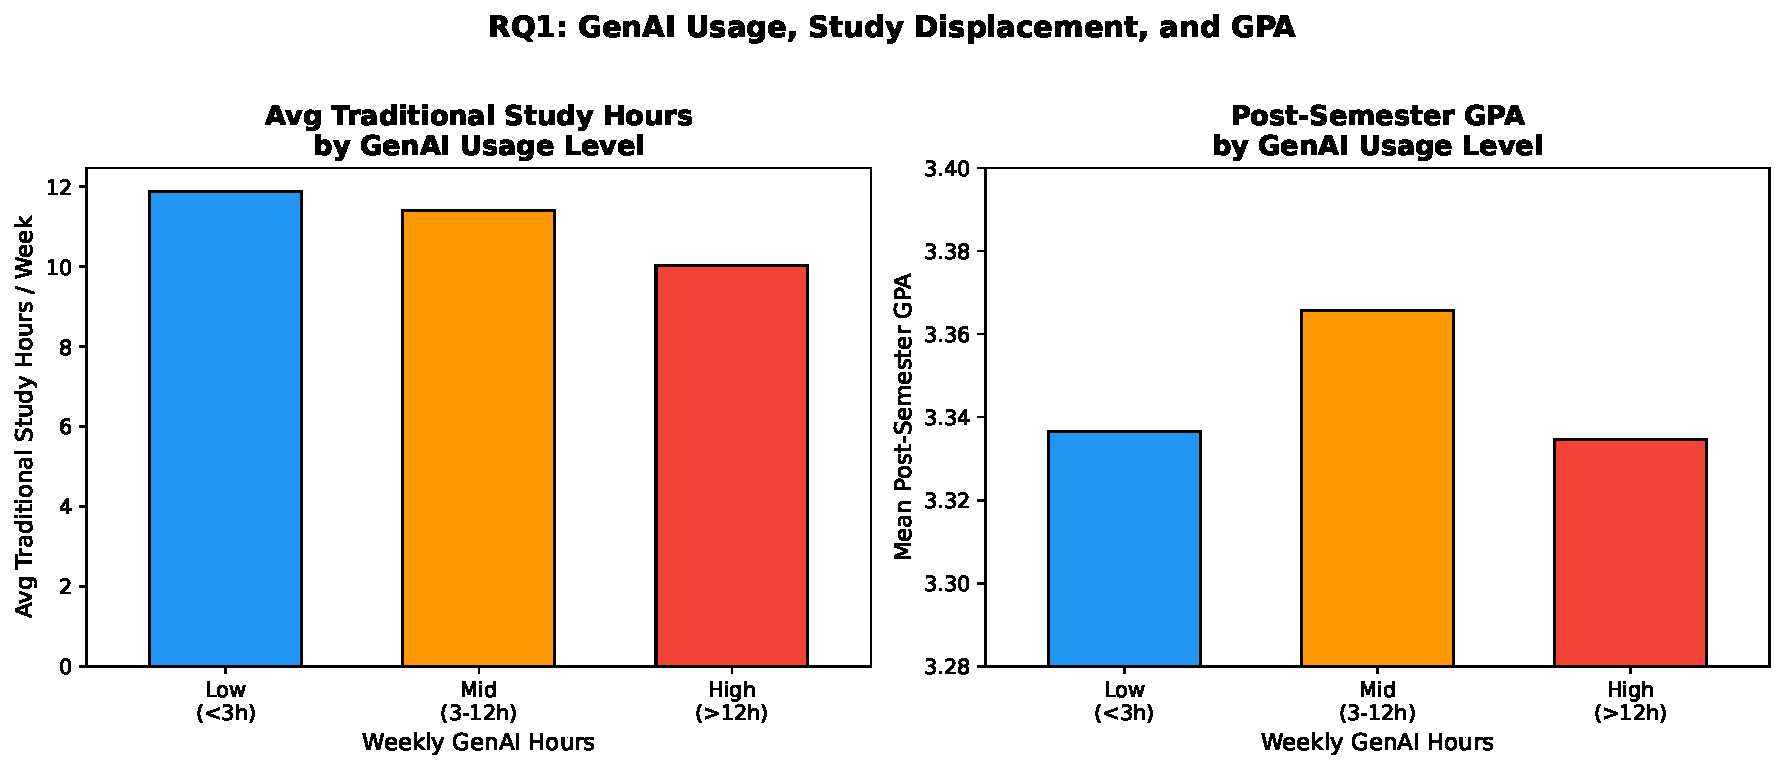
\includegraphics[width=0.92\textwidth]{rq1_genai_study_gpa.pdf}
  \caption{Left: Average traditional study hours fall monotonically with GenAI
    usage. Right: Post-semester GPA peaks in the moderate GenAI bucket,
    consistent with an inverted-U relationship.}
  \label{fig:rq1}
\end{figure}

\subsection*{Interpretation}
Prior GPA dominates post-semester performance ($r = 0.927$), so the direct
GPA effect of AI usage is small in absolute terms. Nevertheless, the statistically
significant non-linear pattern supports the hypothesis that GenAI and traditional
study are partial substitutes: a moderate amount of AI use augments productivity
without crowding out the foundational study time that GPA depends on, whereas
heavy use erodes that base.

%──────────────────────────────────────────────────────────────────
\section{RQ2: Anxiety, Burnout, and Institutional Policy}
\label{sec:rq2}

\subsection*{Findings}

Perceived AI dependency is the strongest single predictor of exam anxiety
($r = +0.308$, $p \approx 0$), followed by weekly GenAI hours
($r = +0.269$, $p \approx 0$). The Kruskal-Wallis test reveals a large and
highly significant difference in anxiety across institutional policies
($H = 667.7$, $p < 10^{-145}$).

\begin{table}[htbp]
\centering
\caption{RQ2: Exam anxiety and burnout by institutional policy}
\label{tab:rq2}
\begin{tabular}{lrr}
\toprule
Institutional Policy & Mean Anxiety (1--10) & High Burnout \% \\
\midrule
Actively Encouraged   & 4.12 & 23.8\% \\
Allowed With Citation & 4.12 & 23.8\% \\
\textbf{Strict Ban}   & \textbf{4.89} & \textbf{29.8\%} \\
\bottomrule
\end{tabular}
\end{table}

Figure~\ref{fig:rq2} shows that Strict Ban environments produce both the highest
mean anxiety (4.89 vs.\ $\approx$4.12) and the highest proportion of students
classified as high-burnout risk (29.8\% vs.\ $\approx$23.8\%).

\begin{figure}[htbp]
  \centering
  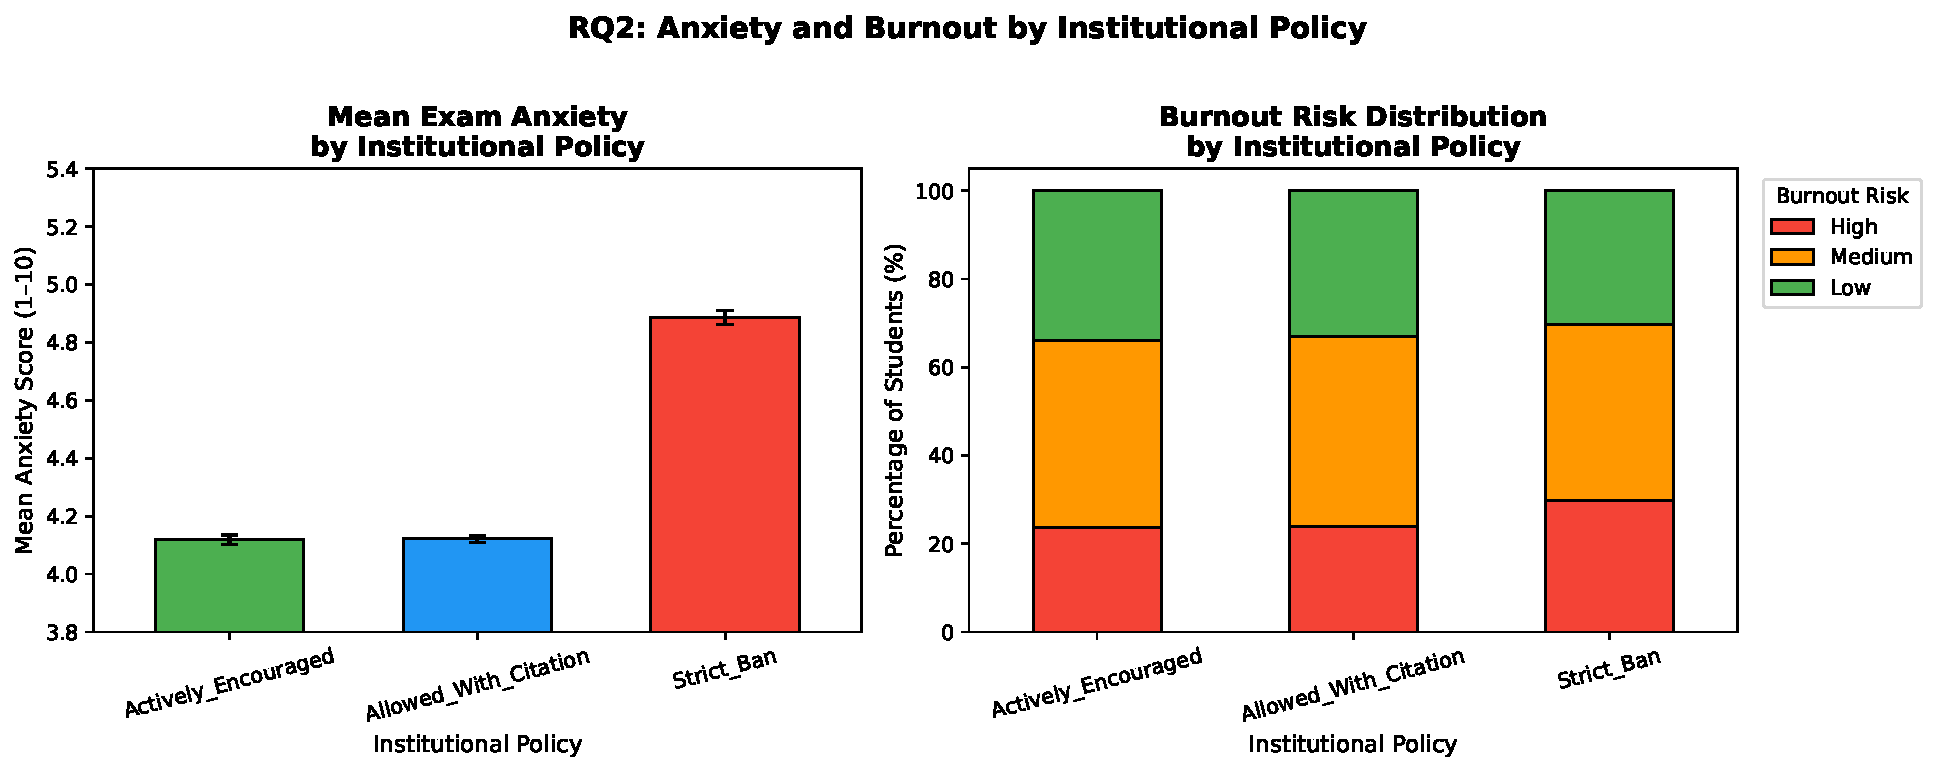
\includegraphics[width=0.92\textwidth]{rq2_anxiety_burnout.pdf}
  \caption{Left: Mean exam anxiety (with standard-error bars) is significantly
    higher under strict AI bans. Right: High-burnout risk is also elevated under
    Strict Ban relative to permissive policies.}
  \label{fig:rq2}
\end{figure}

\subsection*{Interpretation}
The counterintuitive finding is that banning AI \emph{increases} student
anxiety and burnout rather than reducing them. A plausible mechanism is that
students in ban environments continue using AI covertly, adding academic-dishonesty
anxiety on top of ordinary performance pressure. They also lose the productivity
benefit of AI during legitimate study phases, compressing their time budget and
elevating burnout risk. Permissive policies---especially ``Actively
Encouraged''---correlate with the lowest anxiety and burnout, possibly because
transparent guidance reduces ambiguity about acceptable use.

%──────────────────────────────────────────────────────────────────
\section{RQ3: Smart AI Use and Skill Retention}
\label{sec:rq3}

\subsection*{Findings}

Prompt engineering skill is the dominant modifiable predictor of skill retention,
with an 11-point gap between Beginner ($\bar{x} = 71.1$) and Advanced
($\bar{x} = 82.1$) students. One-way ANOVA yields $F = 3012$, $p \approx 0$---
an effect of enormous practical magnitude given the 100-point retention scale.
Tool diversity also exhibits a significant monotonic positive relationship
($r = +0.197$, $p \approx 0$), rising from 72.6 (1 tool) to 79.8 (5 tools)
(Table~\ref{tab:rq3}).

\begin{table}[htbp]
\centering
\caption{RQ3: Skill retention by prompt engineering skill and tool diversity}
\label{tab:rq3}
\begin{tabular}{lrr|lrr}
\toprule
Prompt Skill & Mean & SD & Tools Used & Mean & SD \\
\midrule
Beginner     & 71.10 & 12.67 & 1 & 72.59 & 12.73 \\
Intermediate & 75.83 & 12.43 & 2 & 72.95 & 12.80 \\
Advanced     & 82.05 & 12.53 & 3 & 76.42 & 13.38 \\
             &       &       & 4 & 79.41 & 12.86 \\
             &       &       & 5 & 79.81 & 12.82 \\
\bottomrule
\end{tabular}
\end{table}

Figure~\ref{fig:rq3} shows the interaction of prompt skill with institutional
policy (left panel) and the monotonic tool-diversity effect (right panel).
Institutional policy consistently shifts retention by $\approx 1$ point (Strict
Ban $<$ Allowed $<$ Encouraged), but this gap is dwarfed by the 11-point
skill-level gap. In other words, \emph{how} students use AI matters far more than
\emph{whether} their institution permits it.

\begin{figure}[htbp]
  \centering
  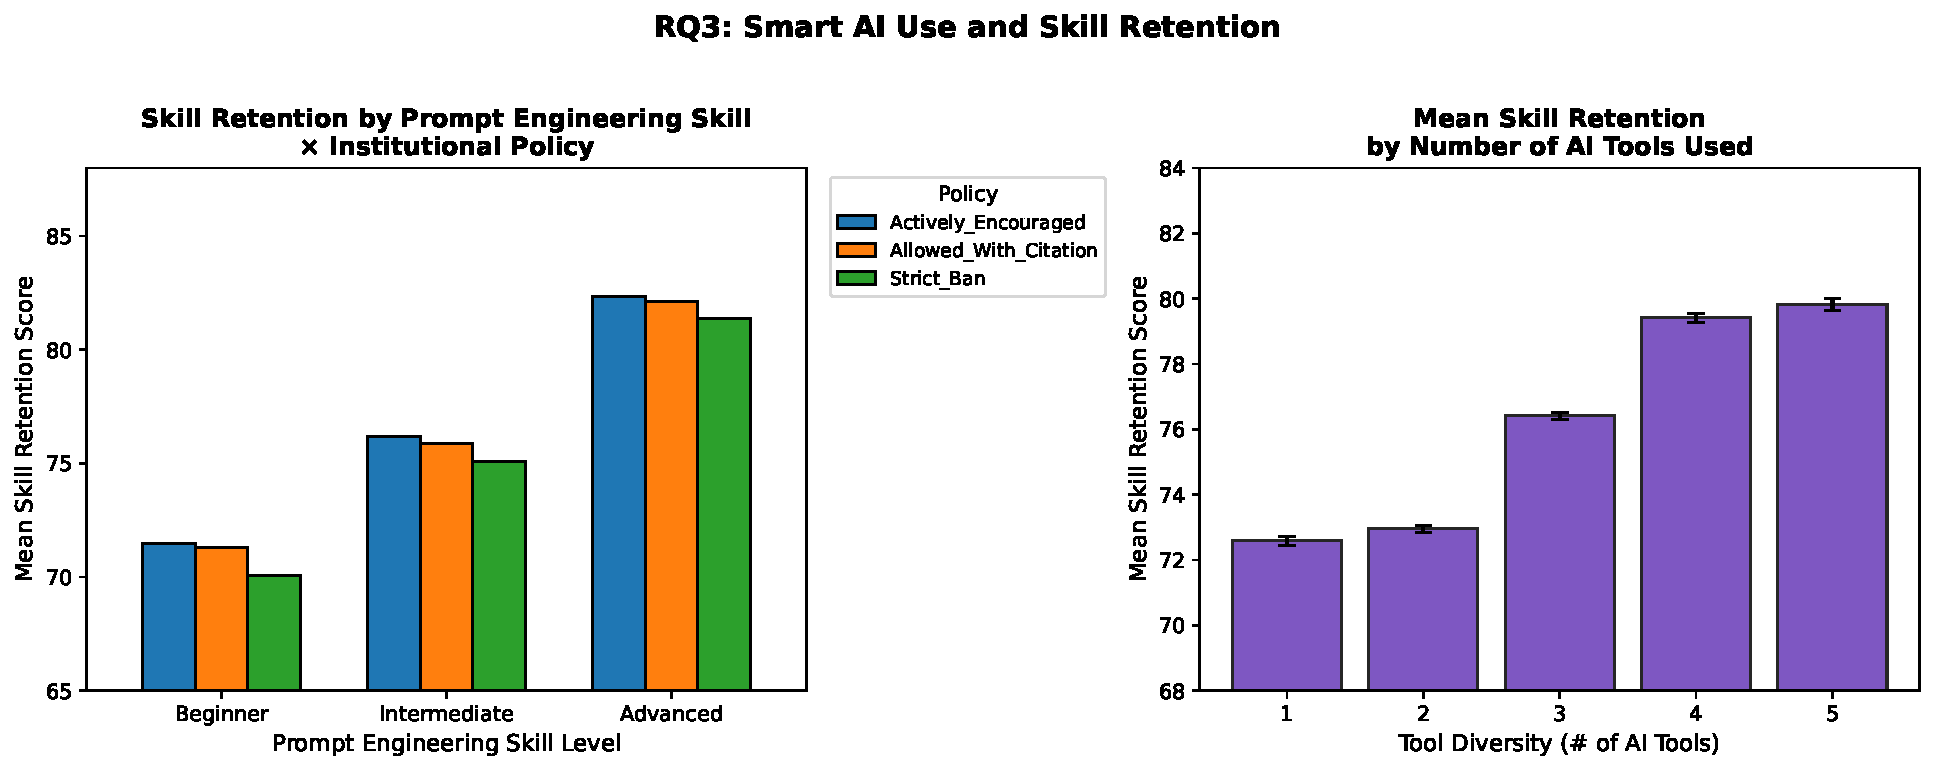
\includegraphics[width=0.92\textwidth]{rq3_retention.pdf}
  \caption{Left: Skill retention rises steeply with prompt engineering skill level
    across all three institutional policies; the ban penalty is modest ($\approx$1
    point). Right: Retention increases monotonically with the number of distinct
    AI tools used.}
  \label{fig:rq3}
\end{figure}

\subsection*{Interpretation}
Students who invest in learning \emph{how} to use AI effectively---formulating
precise prompts, iterating on outputs, and using tools with complementary
strengths---retain substantially more domain knowledge than those who rely on
a single tool with minimal skill. This finding supports a cognitive-augmentation
framing: purposeful AI use that requires active thinking (prompt crafting,
output evaluation) keeps learners engaged with the material, while passive
copy-and-submit use bypasses the consolidation process that drives retention.

%──────────────────────────────────────────────────────────────────
\section{Discussion}
\label{sec:discussion}

\paragraph{Unified picture.}
Across all three RQs, a consistent theme emerges: \emph{quality of engagement
with AI tools outweighs quantity}. Moderate usage optimises GPA; high dependency
drives anxiety; advanced prompt skills dramatically boost retention. The common
thread is metacognitive engagement---students who approach AI as a collaborative
thinking partner rather than an answer machine extract more value at lower
psychological cost.

\paragraph{Policy paradox.}
The burnout and anxiety findings present a cautionary tale for policy-makers.
Strict bans---well-intentioned efforts to preserve academic integrity---appear to
backfire on both the mental-health and learning-outcome fronts. The data suggest
that structured permissiveness (with citation requirements or guided integration)
produces better outcomes than prohibition.

\paragraph{Limitations.}
This is a cross-sectional, observational dataset. Causal claims require caution:
pre-existing differences between students who choose to use AI heavily and those
who do not may confound the estimates. The dataset lacks information on
institution type, country, or socioeconomic background, all of which could
moderate the observed effects. The skill retention metric is not externally
validated against standardised assessments. Future longitudinal work with
experimental variation in institutional policy would substantially strengthen the
causal inference.

%──────────────────────────────────────────────────────────────────
\section{Conclusion}
\label{sec:conclusion}

We set out to understand how generative AI use shapes student academic outcomes
across three dimensions: GPA, mental well-being, and skill retention. The
analysis of 50{,}000 student records yields three actionable conclusions:

\begin{enumerate}
  \item \textbf{Moderate AI use is the sweet spot for GPA.} GenAI and
    traditional study are partial substitutes ($r = -0.16$). Moderate users
    (3--12~h/week) slightly outperform both non-users and heavy users, implying
    a complementarity zone that disappears under excessive use.

  \item \textbf{AI dependency drives anxiety; bans make it worse.} Perceived
    dependency is the strongest predictor of exam anxiety ($r = +0.31$).
    Counterintuitively, institutions with strict bans have 0.77 more anxiety
    points and 6\% more high-burnout students than permissive peers.

  \item \textbf{How you use AI matters more than how much.} Prompt engineering
    skill explains an 11-point retention gap (a large effect), while tool
    diversity adds a further 7 points. These effects vastly exceed the 1-point
    penalty of institutional bans.
\end{enumerate}

\noindent
The practical implication is straightforward: universities should replace
prohibition with structured integration, coupled with deliberate instruction in
prompt engineering and critical AI-output evaluation. Doing so will improve
academic outcomes, reduce anxiety and burnout, and better prepare students for
AI-augmented professional environments.

\end{document}
